\begin{figure}[htbp]
	\centering
	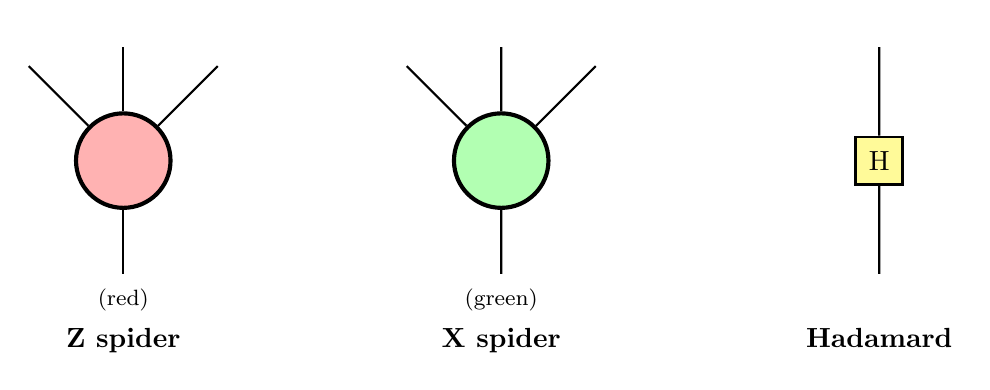
\begin{tikzpicture}[scale=1.2]
		\node[draw, circle, fill=red!30, minimum size=1.2cm, line width=1.5pt] (z) at (0,0) {};
		\draw[thick] (z) -- (0,1.2) node[above] {};
		\draw[thick] (z) -- (0,-1.2) node[below] {};
		\draw[thick] (z) -- (1,1);
		\draw[thick] (z) -- (-1,1);
		\node[below=2.0cm] at (0,0) {\textbf{Z spider}};
		\node[below=1.5cm, font=\footnotesize] at (0,0) {(red)};

		\node[draw, circle, fill=green!30, minimum size=1.2cm, line width=1.5pt] (x) at (4,0) {};
		\draw[thick] (x) -- (4,1.2) node[above] {};
		\draw[thick] (x) -- (4,-1.2) node[below] {};
		\draw[thick] (x) -- (5,1);
		\draw[thick] (x) -- (3,1);
		\node[below=2.0cm] at (4,0) {\textbf{X spider}};
		\node[below=1.5cm, font=\footnotesize] at (4,0) {(green)};

		\node[draw, rectangle, fill=yellow!40, minimum size=0.6cm, line width=1pt] (h) at (8,0) {H};
		\draw[thick] (h) -- (8,1.2) node[above] {};
		\draw[thick] (h) -- (8,-1.2) node[below] {};
		\node[below=2.0cm] at (8,0) {\textbf{Hadamard}};

	\end{tikzpicture}
	\caption{Basic elements of the ZX calculus: Z spiders (red, left), X spiders (green, center), and the Hadamard generator (yellow, right). Spiders are the fundamental building blocks representing quantum states and operations.}
	\label{fig:zx-spiders}
\end{figure}
